

\begin{figure}[h!]
  \begin{center}
    \begin{subfigure}[t]{0.49\linewidth}
      \centering
      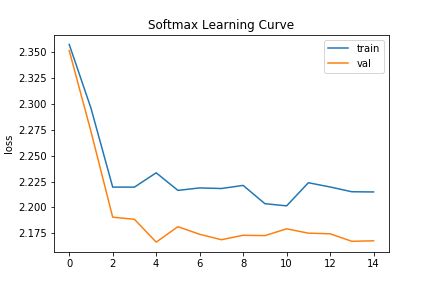
\includegraphics[width=\linewidth]{../code/assignment/2_pytorch/softmax_lossvstrain.png}
      \caption{Evolution of loss during training}
    \end{subfigure}
    \begin{subfigure}[t]{0.49\linewidth}
      \centering
      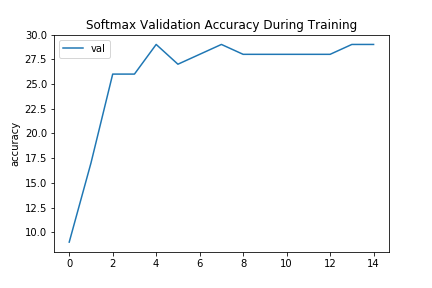
\includegraphics[width=\linewidth]{../code/assignment/2_pytorch/softmax_valaccuracy.png}
      \caption{Evolution of validation accuracy during training}
    \end{subfigure}
    \caption{Evolution of different indicators during training}
  \end{center}
\end{figure}

\begin{figure}[h!]
  \begin{center}
    \begin{subfigure}[t]{0.49\linewidth}
      \centering
      
\includegraphics[width=\linewidth]{../code/assignment/2_pytorch/softmax_gridfilt.png}
        \caption{Filter of the trained softmax model displayed as a grid}
    \end{subfigure}
    \begin{subfigure}[t]{0.49\linewidth}
      \centering
      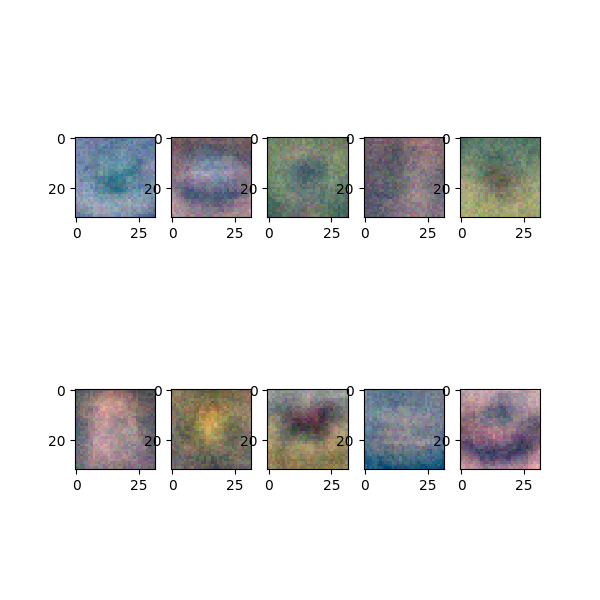
\includegraphics[width=\linewidth]{../code/assignment/2_pytorch/softmax_filt.png}
        \caption{Filter of the trained softmax model}
    \end{subfigure}
    \caption{Weights visualisation after training}
  \end{center}
\end{figure}
